\chapter{Algorithm Details}

The principal goal of the proposed algorithm is to compute
schedules for railway lines (either from scratch or from a given
starting state) while having comparable online computation requirements. 
Three challenges need to be overcome
to in order to achieve this objective

\begin{enumerate}
\item The algorithm must be able to handle different infrastructure and train service instances. 
\item It must scale to large, realistic railway lines.
\item It must manage simultaneously moving trains.
\end{enumerate}
In this approach, the first challenge is addressed by defining a map
from the specific state of the instance to a generalised state
space of fixed size. The second challenge is handled by
decentralising the decisions for individual trains, and limiting
the feature vector to a fixed local horizon around each
train. Finally, the ordering of train moves is handled by
a discrete event simulator which picks the order using a
previously defined deadlock-avoidance heuristic. Each
component is described below.

\vspace{\baselineskip}
Note that this algorithm focuses on computing schedules for \textbf{railway lines instead of railway networks}.
First we will define the algorithm, test it and then have a look at why it can't work in 
railway network setting and then try to expand the learning to the railway network.

\section{Generalised State Representation}
We compute the state space as a function of \textbf{local neighborhood} of each
train.
A state vector is computed for each train every time a
decision about its next move is to be computed. Relative to
the direction of motion, we define resources as being behind
(in the direction opposite to the direction of motion) or in
front (in the direction of motion) of the train. A user-defined
finite number of resources $ l_b $ behind each train and $ l_f $ in
front of each train are used for defining the state vector. These
are referred to as local resources. Including a few resources
behind the train in the state definition ensures that overtaking
opportunities for fast-moving trains are not missed. The total
number of local resources is ($ l_b + 1 + l_f $). 

\vspace{\baselineskip}
The entry in the state vector corresponding to each local
resource takes one of R integer values $ \{0, 1, 2,..., R-1\} $,
referred to as the status $S_r$ of resource $r$. Higher values
indicate higher congestion within the resource, and are driven
by the number of occupied tracks.
Let us define the number
of tracks in resource r to be equal to $N_r$, out of which $T_{r,c}$
tracks contain trains converging with (heading towards) the
current train, while $T_{r,d}$ tracks contain trains diverging from
(heading away from) the current train. Since at most one train
can occupy a given track, we note that $T_{r,c} + T_{r,d} < N_r$. The
mapping from track occupancy to resource status is,

$$ S_r = R - 1 - min(R - 1, \left \lceil{N_r - w_c T_{r,c} - w_d T_{r,d} }\right \rceil ).$$

Here, $0 \leq w_c$, $w_d \leq 1$ are weights that can de-emphasise
the effect of converging and diverging trains on the perceived
status of a resource.

\vspace{\baselineskip}
In addition to the resource-related entries, the state includes
an entry for the priority of the current train.

\vspace{\baselineskip}
The complete state representation
used is a vector x of length ($l_b + l_f + 2$), including
the integer priority value and ($l_b + 1 + l_f$) entries for the status
of local resources. If we assume that the model accommodates
up to $P$ priority levels, the size of the state space is equal to
\textbf{($P * R^{l_b + 1 + l_f}$)}.\textbf{Note that this value does not depend on the
scale of the problem instance, in terms of the number of trains,
the lengths of their journeys, and the number of resources}.
One of the key advantage of using the local horizon as the state for the train is it's independence 
from the size of the problem instance. Another advantage is of \textbf{transfer learning} which we will see in later
sections.

\section{Action and Policy Definition}
The reinforcement learning procedure maps each state vector
 to a probability of choosing the action to be taken. In this
study, the choice of actions in any given state is binary, with
0 representing a decision to move the current train to the next
resource on its journey, and 1 representing a decision to halt
in the current resource for a predefined time period (1 minute
in this paper). If the train is halted, the decision-making
procedure is repeated after the time period elapses. The order
in which trains are selected for move/halt decision-making is given 
by deadlock avoidance heuristic in resource usage module. Let us assume that
a particular train occupying one track of some resource $r$ has
been selected, the state vector has been computed, and the
action (move or halt) is to be chosen. In addition to the state
vector, the choice of action is driven by the policy. Policy depends on the approach that we are going to use. 

\subsection{ $\epsilon$ - greedy policy}
Given a state, the two possible actions $a \in$  $\{$0 : move, 1 : halt$\}$ result in two unique
state-action pairs. Each state-action pair (x, a) is associated
with a Q-Value q(x, a) which quantifies its desirability. The higher the Q-Value, the higher the
desirability of the relevant pair. The $\epsilon$-greedy policy chooses
the greedy option (higher Q-Value) with probability ($1 - \epsilon$),
and a randomised action with probability $\epsilon$. The greedy choice
corresponds to \textbf{exploitation} of the learning so far, while the
randomised choice corresponds to \textbf{exploration} of the state-
action space. We are going to use this policy with standard Sarsa$(\lambda)$ the results of 
which are not good.

\subsection{Modified $\epsilon$ - greedy policy}

\begin{figure}[h]
    \centering
    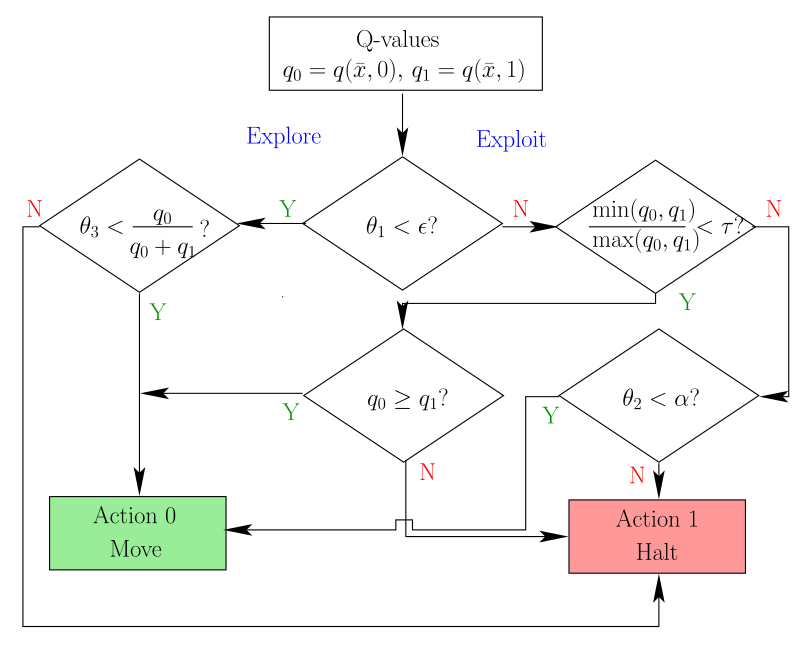
\includegraphics[width=0.7\textwidth]{policy}
    \caption{ Modified greedy policy }
    \label{image-myimage20}
\end{figure}

This is a modified version of the $\epsilon$ - greedy policy.
In exploration mode, the action is chosen with the
toss of a biased coin, based on the relative Q-Values $q_0$ and $q_1$
of the two actions. In the exploit mode, if $q_0 \approx q_1$
within a user-defined threshold $\tau$ , a further biased coin toss
is used to compute the action. The bias in this case is given
by a user-defined aggression parameter $\alpha$, which controls the
probability of choosing ‘move’ when $q_0 \approx q_1$ . If $q_0$ and $q_1$
are clearly separated, the action with the higher Q-Value is
chosen. The value of $\epsilon$ starts at 1 in the first training episode
and decreases as more episodes are completed. This moves
the policy gradually from exploration towards exploitation.

\vspace{\baselineskip}

The value of $\epsilon$ remains the same throughout the whole episode. In the first episode 
$\epsilon = 1$ and as the episode passes the value of epsilon decreases linearly upto min $\epsilon$,
after which it remains constant throughout the whole training.

\section{Objective Function}
A number of objective functions have been used in the
railway scheduling context, in order to achieve goals such
as delay reduction, passenger convenience, and timetable
robustness. One of the commonly used measures of
schedule quality is priority-weighted delay. A delay is
defined to be the non-negative difference between the time
of an event as computed by the algorithm, and the desired
time as specified by the timetable. The priority-weighted
average delay is the mean over all trains and all stations
of individual delays divided by train priorities. This quantity
is used as the objective function, but the algorithm can
accommodate other measures equally easily (for example,
a non-linear function of delays in order to increase fairness
of delay distribution).
$$ J = \frac{1}{N_{r,t}} \sum_{r,t} \frac{\delta_{r,t}}{P_t} $$
where $\delta_{r,t}$ is the delay for train t on departure from resource r,
$p_t$ is the priority of train t, and $N_{r,t}$ is the total number of
departures in the schedule. Note that this expression includes
all events for all trains, for their entire journey.

\section{Sarsa$(\lambda)$}
One of the typical algorithm is to use the objective function defined above as the negative of the reward. 
In that case, we will be having the reward at the end of each episode (terminal episode).
In each episode, each train is going through certain state-action pairs, forming a trajectory. And at the end
of each episode, we will get the reward. We can backpropogate the reward through this trajectory to learn
the Q-values. This learning is done using Sarsa($\lambda$).

\vspace{\baselineskip}
In Sarsa($\lambda$), we are using standard $\epsilon$ - greedy policy. This section discusses the forward view of 
Sarsa ($\lambda$) using eligibility traces. Q-values are updated using 
$$ Q_{t+1}(s,a) = Q_t(s,a) + \alpha\delta_te_t(s,a)  \;\; \forall(s,a)$$ 
where 
$$\delta_t = r_{t+1} + \gamma*Q_t(s_{t+1} , a_{t+1}) - Q_t(s_t ,a_t)$$
and 
\[
    e_t(s,a)=\left\{
                \begin{array}{ll}
                  \gamma\lambda e_{t-1}(s,a) + 1 \;\; if \; s=s_t \;\; and \; a=a_t\\
                  \gamma\lambda e_{t-1}(s,a) \;\;\;\;\;\;\;\; otherwise.\\
                \end{array}
              \right.
\]

Here, $\alpha$ is the learning rate, $\gamma$ is discount factor, $r_{t+1}$ is the reward (we have only 
one reward at the end of episode). Algorithm is given below.
\vspace{\baselineskip}

The results of this algorithm is not good (in the next section) due to following reasons,
\begin{enumerate}
\item The back-propagation of rewards
      after the end of the episode is not possible, because the episode
can be very long.
\item In the trajecotry of a train, it is possible to visit the same state-action pair in loop leading to 
large accumulation of reward at that state-action pair, leading to extreme values.
\item Moreover, the magnitude of delays (and hence the theoretical
optimum value of $J$ ) is different from one problem instance
to another. Quantifying rewards directly in terms of delays
$\delta_{r,t}$ would create obstacles when transferring the learning from
one instance to another (\textbf{obstacle in transfer learning}).
\end{enumerate}
\begin{figure}[!htb]
    \centering
    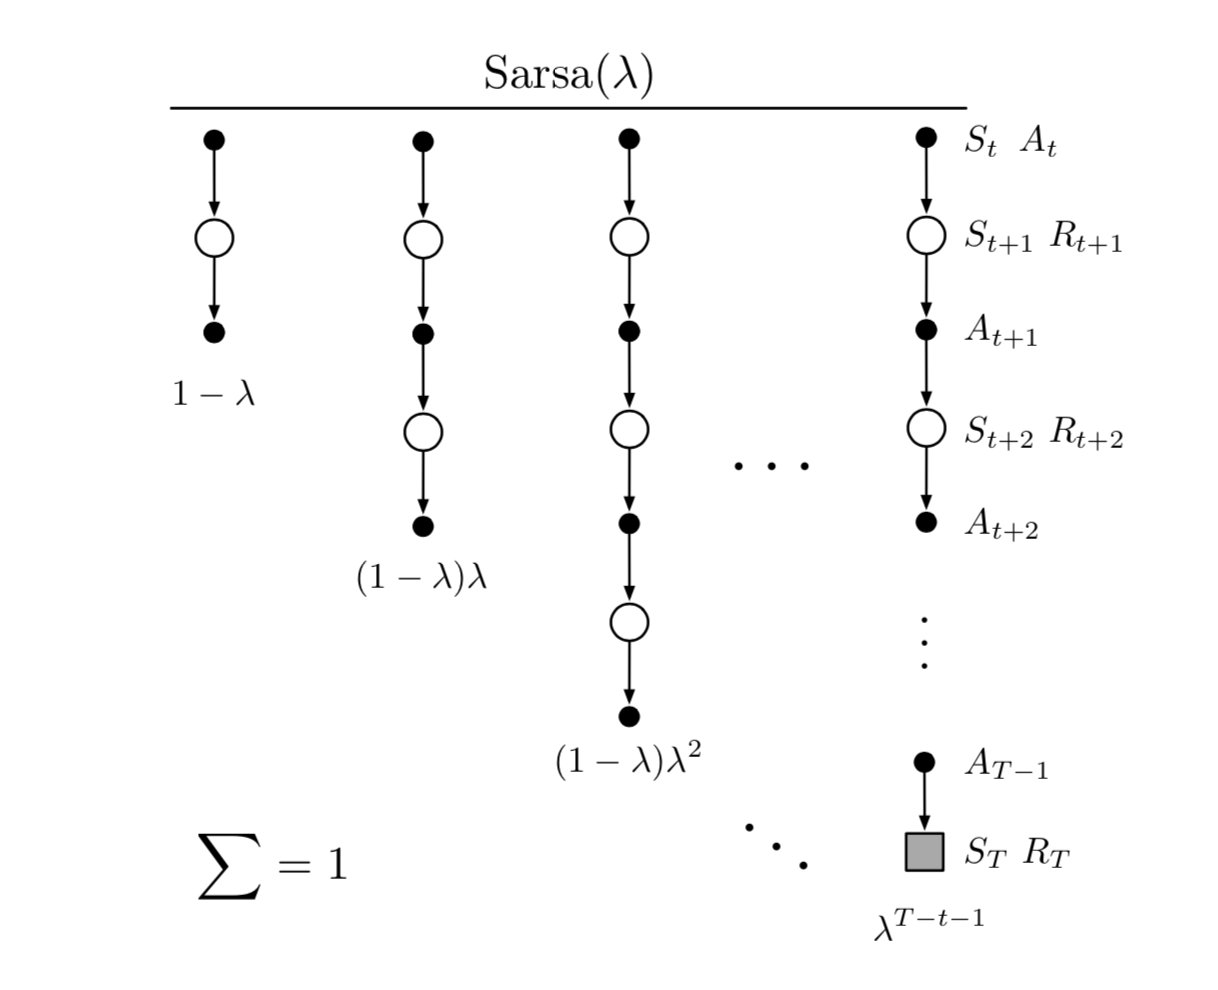
\includegraphics[width=0.7\textwidth]{backup_sarsa}
    \caption{ Sarsa($\lambda$)'s backup diagram }
    \label{image-myimage20}
\end{figure}

\begin{algorithm}[H]
\caption{ Sarsa Lambda }
\begin{algorithmic}
\State Initialize $Q(s,a)$ arbitrarily and $e(s,a) = 0$ $\forall s,a$
\State Repeat (for each episode):
\State \;\;\;\;\;\;Initialize s,a    
\State \;\;\;\;\;\;Repeat (for each step of episode):
\State \;\;\;\;\;\;\;\;\;\;\;\; Take action $a$, observe $r$,$s'$
\State \;\;\;\;\;\;\;\;\;\;\;\; Choose $a'$ from $s'$ using $\epsilon$ - greedy policy
\State \;\;\;\;\;\;\;\;\;\;\;\; $\delta \gets r + \gamma Q(s',a') - Q(s,a)$
\State \;\;\;\;\;\;\;\;\;\;\;\; $e(s,a) \gets e(s,a) + 1$
\State \;\;\;\;\;\;\;\;\;\;\;\; For all $s$,$a$
\State \;\;\;\;\;\;\;\;\;\;\;\;\;\;\;\;\;\; $Q(s,a) \gets Q(s,a) + \alpha \delta e(s,a)$
\State \;\;\;\;\;\;\;\;\;\;\;\;\;\;\;\;\;\; $e(s,a) \gets \gamma \lambda e(s,a)$
\State \;\;\;\;\;\;\;\;\;\;\;\; $s \gets s'; a \gets a'$
\State \;\;\;\;\;\; until s is terminal
\end{algorithmic}
\end{algorithm}


\section{Proxy reward}

The algorithm maintains a threshold of $J$ as the goal to be
achieved in each episode. This maximum acceptable level is
set to a proportion (1 + $\rho$) of the minimum $J$ observed thus
far, where $\rho > 0$ is a user-defined constant. The threshold
becomes tighter as the best known $J$ is improved upon during
learning. A reward of +1 (success) is given if the sum of the
priority-weighted delay is under the current threshold, and 0
(failure) either if it is over the threshold, or if the episode
enters deadlock and does not terminate.

The Q-Values
are defined using the probability of success when an episode
passes through a given state-action pair. Instead of tracking
the entire sequence of state-action pairs in a given episode,
a binary indicator variable $b( x, a)$ corresponding to each pair
$( x, a)$ is set to TRUE whenever it is observed in a given
episode. Upon termination of the episode, the number of
successes (or failures) of all ( x, a) where $b( x, a) = TRUE$
are incremented by 1. The success probability $\sigma ( x, a)$ is
computed by dividing the number of +1 rewards associated
with the pair, by the total number of episodes that passed
through this pair. If $\epsilon_{x,a}$ is the number of all episodes that
passed through (x, a) at least once, and $\epsilon^{*}_{x,a}$ is the number of these 
that ended in success,
$$ 0 \leq \sigma(x,a) = \frac{\epsilon^{*}_{x,a}}{\epsilon_{x,a}} \leq 1$$

While $ \sigma ( x, a)$ provides a way to quantify the desirability
of a given state-action pair, it does not encapsulate the state
trajectory. On the other hand, a core tenet of reinforcement
learning is the back-propagation of rewards through the trajectory of state-action pairs (usually
upon episode termination).
However, in the current context, episodes can be very long,
reward is generated only upon episode termination, and state-
action pairs for multiple trains are generated simultaneously.
Therefore, $\sigma ( x, a)$ is used in as a \textbf{proxy reward}.

In the paper, Q-value is defined as 
$$ q(x,a) = w\sigma(x,a) + (1-w)\sum_{m=1}^{M}\frac{\sigma(x'_m, a'_m)}{M }  $$
where $w$ is the weighing factor, $(x'_m, a'_m)$ are the neighbors (say M) of $(x_m,a_m)$ during an 
episode. 